\chapter{Breve historia de mi vida}

Hola soy Martin, actualmete  fui aceptado en la facultad de Ciencias en la carrera de Ciencias de la computacion, naci el 9 de agosto de 1999, y he pasado casi toda mi vida en la Ciudad de México a ecepción de un par de años que viví en púebla

\begin{figure}[h]
  \centering
  
\includegraphics[scale=0.5]{IMG/19_2.jpg}
  \caption{Facultad de ciencias}
  \label{fig:facultad}
\end{figure}


\chapter*{Mi familia}

Mi padre se llama MIguel Ángel, y mi madre se llama Sandra Lisbeth; Tengo 2 hermanos, mi hermano mayor se llama Josue y mi hermana menor se llama Ana

\begin{figure}[h]
  \centering
  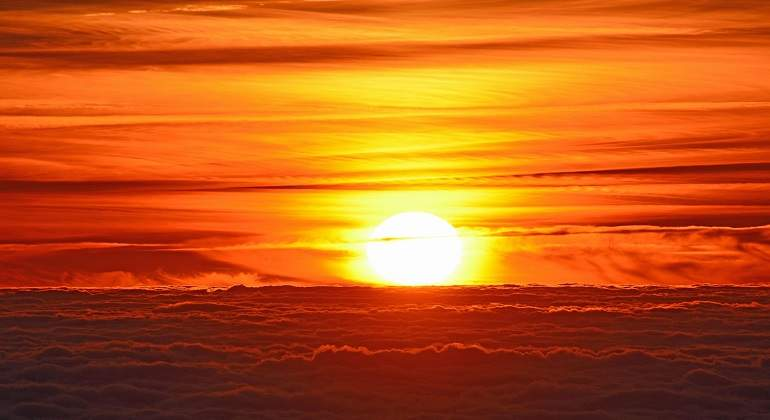
\includegraphics[scale=0.5]{IMG/19_4.jpg}
  \caption{Atardecer}
  \label{fig:atardecer}
\end{figure}


\chapter*{Mis gustos}

Me gustan las matemáticas ya que son bastantes entretenidas y en ellas encuentro muchos retos interesantes
\begin{itemize}
\item $c^2 = a^2 + b^2$
\item $x=-b \pm \frac{\sqrt{b^2-4ac}}{2a}$
\end{itemize}


\begin{table}[h]
  \centering
  \begin{tabular}{| c  c  c  |}
    \hline
    Operando & Operando & Resultado\\\hline
    $+$ & $+$ & $+$\\\hline
    $+$ & $-$ & $-$\\\hline
    $-$ & $+$ & $-$\\\hline
    $-$ & $-$ & $+$\\\hline    
  \end{tabular}
  \caption{Leyes de los signos}
  \label{tabla:leyes_signos}
\end{table}

Tambien me agrada bastante la música del anterior siglo
\begin{figure}[h]
  \centering
  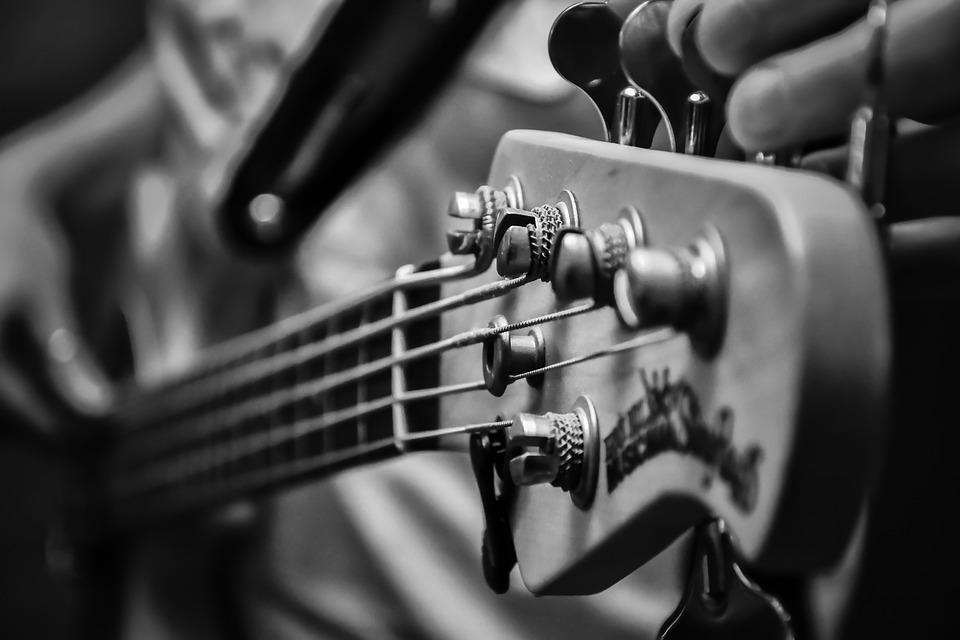
\includegraphics[scale=0.5]{IMG/19_1.jpg}
  \caption{iamgen de lo que me gustaria aprender}
  \label{fig:guitarra}
\end{figure}

\chapter{Mis planes}

Planeo terminar mi carrera, conseguir un buen empleo, administrar mi tiempo para continuar con estudios de pos grado, e intentar ser feliz-

\begin{figure}[h]
  \centering
  
\includegraphics[scale=0.5]{IMG/19_3.jpg}
  \caption{ciencias de la computacion}
  \label{fig:computo}
\end{figure}




